%%%%%%%%%%%%%%%%%%%%%%%%%%%%%%%%%%%%%%%%%%%%%%%%%%%%%%%%%%%%%%%%%%%%%%%%%%%%%%%%%%%
% Team:
% Union
% Members: 
% Bernie Huan, Jim Lan, Hoang Tan, Kenny Hsu, Rahul Aditya, Tan Phat, Wei
% Relative files:
% Main.tex, Background_Union.tex, Library.bib, Union_Background_Chart_1.png, Union_Background_Chart_2.png, Union_Background_Chart_3.png, Union_Background_Chart_semi.png, Union_Background_Chart_sup1.png, Union_Background_Chart_sup2.png, Union_Background_Chart_sup3.png, Union_Background_Chart_WSD.png
% Note:
% Do not compile this file compile Main.tex to get the pdf file instead.
%%%%%%%%%%%%%%%%%%%%%%%%%%%%%%%%%%%%%%%%%%%%%%%%%%%%%%%%%%%%%%%%%%%%%%%%%%%%%%%%%%%

\subsection{Automatic creation of metadata}
\textit{\footnotesize Author:Bernie Huan, Jim Lan, Hoang Tan, Kenny Hsu, Rahul Aditya, Tan Phat, Wei.}\\

We are producing a program that automatically generate metadata. Threre are three main subjects we want to extract: authors' name, title and abstract of the article .\todo{Please update based on what you are building}

We are interested in features for either more convenient uses of the program or improving precise data generation.There are 5 related problems.

\begin{figure*}[ht]
	\begin{center}
		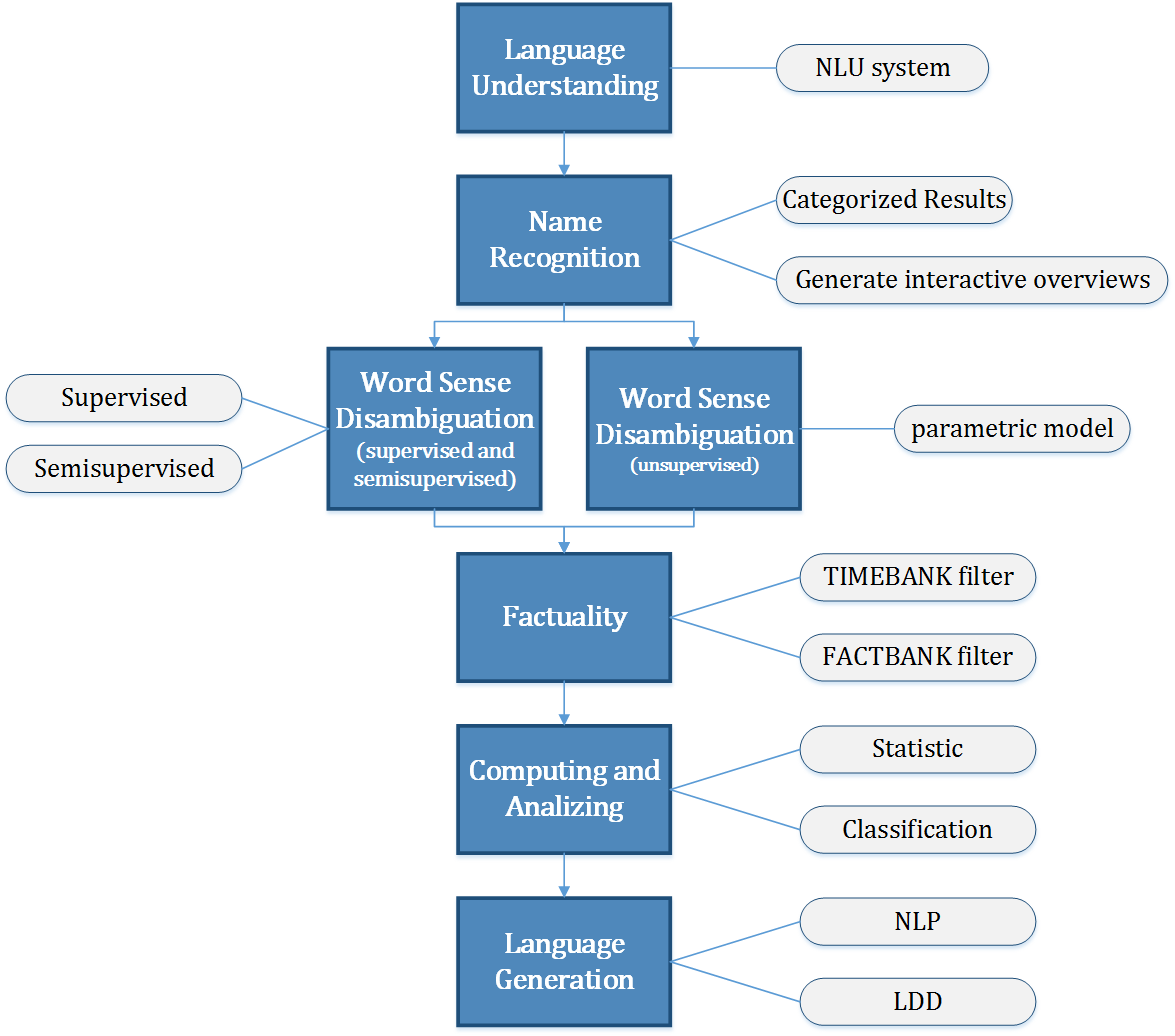
\includegraphics[width=1.8\columnwidth]{Union_Background_Chart_1}
	\end{center}
\caption{The process of metadata creation.}
\end{figure*}

\subsubsection*{Language understanding}
When users search for a sentence, how does the program understand certain inputs of text? 

We can build a natural language understanding (NLU) system, which uses a set of possible yes-no questions that can be applied to data items. \todo{What is an NLU system? Questions about what? What is a node? Why a tree? Add more material to make it understandable. Add citation of a review of NLU.} After that, it follows rules for selecting the best question at any node on the basis of training data by using a method for pruning trees to prevent over-training.

\todo[inline]{I believe you should read some publication and cite their work properly. Clarity in your writing should also be improved.Please take a look at it (Phat's comment)}

\subsubsection*{Name Recognition}

The results could be a country or an animal if users search for the word, Turkey. The type (meaning instead of type) is very different.

There are a lot of misunderstandings like this if users search some words which have multiply meanings. Sometimes, the results are totally unrelated and this situation is always annoying. That would be troublesome when we count frequency of certain words to rank them.
 
Therefore, it is significantly crucial for a program to totally understand what users want by name recognition in natural language processing. The users can find out the results much quicker and can't get misunderstood (and will not be confused?).

The method to improve the problem above is "categorize the words based on different subjects,topic or genres" by using online database. Metadata is limited in digital libraries and web resources, try to enlarge them with meaningful, organized and desired categories \cite{Kules2006}.
Besides dealing with mutiple-meaning words,the most important part of name recognition is to recognize the special names and terms such as locations,people name,even company names and academic terms. Therefore, it is better for search engine to know what user want and huge name corpus are necessary. Plus, this work also can assist previous work.



With above effort,users' exploration and overviews of information could be better supported. It will be very convenient to find the results we want and lower the possibility of misunderstanding if users are not very familiar with finding the appropriate result in specific fields.\cite{TunThuraThet2010} Users don not have to filter the results which are ranked by browsing frequency popularity. Users just can obtain the information and relevance by clicking the specific categories. Also, users are able to choose multiply fields if the results include a lot of relevant fields. That's a big motivation for people to handle this problems. 

A lot of online services have done similar tasks before .Thus,creating and using an online database or automated metadata creation are to be recommended. \todo{Citation or a few examples needed.} The reason is there are many advantages, including integrating with the other cloud services or scaling with what users need such as how to categorize the categories. It is beneficial for people who would like to create a convenient and personalized database or metadata.\\

\subsubsection*{Word sense disambiguation: supervised and semi-supervised approach}

\begin{figure}[tbh]
	\begin{center}
		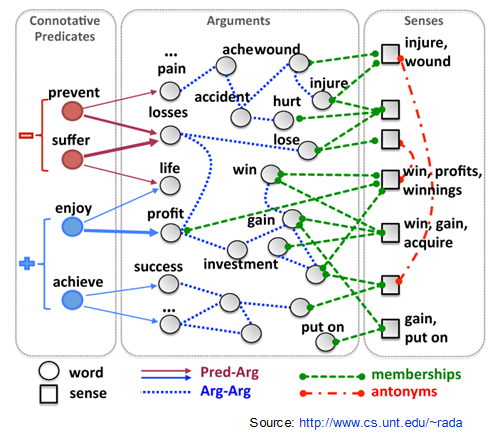
\includegraphics[width=\columnwidth]{Union_Background_Chart_WSD}
	\end{center}
	\caption{GWord+Sense with words and senses. \label{fig1}}
\end{figure}

Word sense disambiguation (WSD) is an open problem of natural language processing and ontology. WSD identifies which sense of a word (i.e.meaning) is used in a sentence, when the word has multiple meanings \cite{Du2013}. The solution to this problem impacts other computer-related writing, such as discourse, improving relevance of search engines, anaphora resolution, coherence, inference et cetera.

Word Sense Disambiguation(WSD) is related to Natural Language Processing and is also linked with computational languages. People introduced it as a solution when they felt the need of some complex problems like machine translation, information retrieval, speech processing and text processing etc. WSD is mainly focused on determining the sense of word,computationally which is used in a problem by using that word in a particular context. Inspite of having a greater number of existing disambiguation algorithms, WSD still has an open problem with the three main parts of the WSD methods being considered by literature: Supervised, Unsupervised and semi-supervised. \todo{Merge this text into the rest in this section. I moved it from another place.}

The human brain is quite proficient at word-sense disambiguation. The fact that natural language is formed in a way that requires so much of it is a reflection of that neurological reality. In other words, human language developed in a way that reflects (and also has helped to shape) the innate ability provided by the brain's neural networks. In computer science and the information technology that it enables, it has been a long-term challenge to develop the ability in computers to do natural language processing and machine learning. \todo{Why not insert a figure showing how the best solution has improved over time and how many solutions that exist?}

\subsection*{Supervised}

\begin{figure}[tbh]
	\begin{center}
		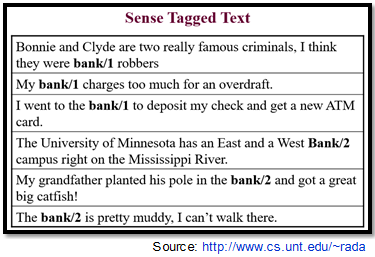
\includegraphics[width=\columnwidth]{Union_Background_Chart_sup1}
	\end{center}
	\caption{Sense tagged text.}
\end{figure}
\begin{figure}[tbh]
	\begin{center}
		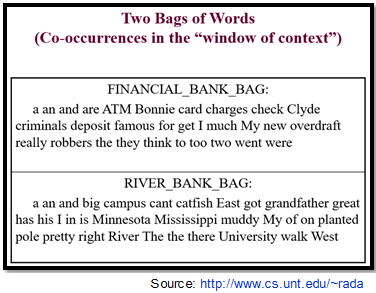
\includegraphics[width=\columnwidth]{Union_Background_Chart_sup2}
	\end{center}
	\caption{Two bags of words.}
\end{figure}
\begin{figure}[tbh]
	\begin{center}
		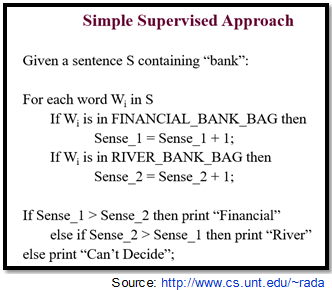
\includegraphics[width=\columnwidth]{Union_Background_Chart_sup3}
	\end{center}
	\caption{Supervised approach.}
\end{figure}

Supervised methods are based on the assumption that the context can provide enough evidence on its own to disambiguate words. Probably every machine learning algorithm going has been applied to WSD, including associated techniques, such as feature selection, parameter optimization, and ensemble learning.\todo{Try to avoid speculations. If you speculate you should motivate it.} Support Vector Machines and memory-based learning have been shown to be the most successful approaches, to date, probably because they can cope with the high-dimensionality of the feature space. However, these supervised methods are subject to a new knowledge acquisition bottleneck since they rely on substantial amounts of manually sense-tagged corpora for training, which are laborious and expensive to create \cite{aramossoto2016onthe}.

\subsubsection*{Semi-supervised}

Because of the lack of training data, many word sense disambiguation algorithms use semi-supervised learning, which allows both labeled and unlabeled data. The Yarowsky algorithm was an early example of such an algorithm \cite{Gartner201317}. It uses the 'One sense per collocation' and the 'One sense per discourse' properties of human languages for word sense disambiguation. Based on observation it has been shown that words tend to exhibit only one sense in most given discourse and in a given collocation. \todo{Good beginning. An example or explanation of the properties is needed. A citation on the last sentence is needed.}

\begin{figure}[tbh]
	\begin{center}
		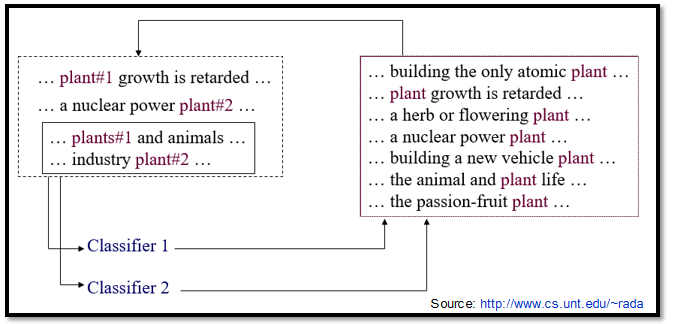
\includegraphics[width=\columnwidth]{Union_Background_Chart_semi}
	\end{center}
	\caption{Classifier that improves over the basic classifier. \label{fig3}}
\end{figure}

The bootstrapping approach\todo{Which bootstraping? Missing text in between.} starts from a small amount of seed data for each word: either manually tagged training examples or a small number of surefire decision rules. The seeds are used to train an initial classifier, using any supervised method. This classifier is then used on the untagged portion of the corpus to extract a larger training set, in which only the most confident classifications are included. The process repeats, each new classifier being trained on a successively larger training corpus, until the whole corpus is consumed, or until a given maximum number of iterations is reached \cite{Blascheck2016}.

Other semi-supervised techniques use large quantities of untagged corpora to provide co-occurrence information that supplements the tagged corpora. These techniques have the potential to help in the adaptation of supervised models to different domains.

Also, an ambiguous word in one language is often translated into different words in a second language depending on the sense of the word. Word-aligned bilingual corpora have been used to infer cross-lingual sense distinctions, a kind of semi-supervised system\cite{Cheslow2014}.

\subsubsection*{Unsupervised}

Unsupervised WSD which rely on single writing can be approached by the use of Naive Bayes' model, which mainly focuses on unsupervised part of the context. In this model, a number of sentences are used which contains a particular word which has several meanings. The main goal is to divide those words into a specified number of sense groups \cite{4028513}.
The Naive Bayes model applied mathematically entirely focuses on the issue of feature selection, which describes its two types:

\begin{enumerate}
	\item Pedersen and Bruce local type features.
	\item WordNet-based feature selection.
\end{enumerate}

\begin{enumerate}
	\item Pedersen and Bruce local type features:
\end{enumerate}
Three different feature sets have been used by 'Pedersen and Bruce' (under Naive Bayes model) for each word to formulate such a model describing the distributions of sense groups of that word in Unsupervised WSD.

The features which were taken into account are:
\textbf{Morphology:} The pattern of word formation in a particular language is called as Morphology.This feature represents the morphology of the ambiguous word and is denoted by M.In case of nouns, M acts as Binary which indicates whether the word is plural or singular.For verbs, M indicates the tense of the verb and can have up to seven possible values.This feature is not applicable for adjectives.

\textbf{Part-of-speech:} This feature represents the part-of-speech of the word and tells the position of the ambiguous word.Each POS feature can have one of five possible values: noun, verb, adjective, adverb or other.

\textbf{Co-occurences:} This feature also acts as binary variables representing whether the most frequent content word in all the sentences contains the ambiguous word can occur anywhere in the sentence or not.

Apart from the above mentioned model, the web can act as a corpus too, where it searches words which are relevant and distinctive for the target word, which makes it more appropriate in searching particular words' meaning.

So, this background focuses mainly on the issues of feature selection for unsupervised WSD performed with an underlying Naive Bayes model.\todo{Really? This section is shorter.}

The difference between 'Supervised' and 'Unsupervised' WSD is:

\begin{enumerate}
	\item The Supervised WSD approach requires a large amount of data in order to achieve a reliable result and generally the scope is limited to some words. Whereas the Unsupervised WSD approach does not use any corpus and suggests the suitable information extracted to the word knowledge base.This method is used in case of performing WSD without data learning.
	\item The Supervised approaches make use of information from labeled training data while the Unsupervised does not depend upon any labeled data, it uses a multi-lingual thesaurus that contains millions of biomedical and health related concepts, their synonymous names and their relationships.
\end{enumerate}
\todo[inline]{A summary on list format can be motivated, but then each item need to be brief and you should not introduce anything new like UMLS in it.}

\subsubsection*{Factuality}

In the process of producing metadata\todo{Data is plural, so you cannot write datas}, which are should be the most precise information and representing the text, validity of such metadata must be checked. Therefore tools for fact checks are developed based on linguistic techniques. The tool could detect facts and excludes authors' subjective opinions \cite{Agerri2014}. From this paper's perspective,\todo{A paper cannot have a perspective, but the authors of a paper can.} the two main set of tools having such functions is TIMEBANK and FACTBANK.\todo{Did the authors always use capital letters? If not treat them as names, so only the first letter should be capital.}

TIMEBANK was first proposed in \cite{pustejovsky2003timebank}. The idea was based on that English language has different tenses which could be exploited as signals for fact check. An example as below could help to clarify the ideas. Let's examine these sentence:

\begin{itemize}
	\item I will go to Chimei museum tomorrow.
	\item Chimei museum is near Tainan District.
	\item I was in UK in 2012.
\end{itemize}

The first sentence is simple future tense which imply something has never actually happened, the second sentence is simple present tense which can directly imply facts, and the last sentence is in simple past tense which is about something already happened (which is facts), but is no longer a fact right now -- so such fact must be used with caution. 

In addition to TIMEBANK, many other tools can be another filter for fact extraction.\todo{Give a few examples.} The reason for introducing such tool is that even scientific research articles can be glittering with subjective comments, opinions or even assumption from authors \cite{schultze2000confessional}. \cite{Dave2003mining} identify words, clauses and phrases that show emotional state of the authors. The choice in expression of facts could also be a helpful indicator to show whether authors are subjectively supporting a cause, an opinion and so on \cite{Wiebe2005}. Among these mentioned approaches, this paper highly favors creation a kind of thesaurus compiled of linguistic signaling for non-factually statements such as FACTBANK, which is built by \cite{Sauri2009}. Following example shows how subjective statements can be picked out.

\begin{itemize}
	\item Channelization would guarantee high flow velocity in rivers, more flooding and consequent degradation of riparian community (1a)
	\item Funding agencies would be happy with big entrepreneurs, instead of small and medium enterprises. (1b)
	\item Tolerance to dictatorship would has negative influences on anarchist movement (2a)
	\item Tolerance to dictatorship would doom anarchist movement. (2b)
\end{itemize}
\todo{Punctuation should be fixed.}

It is easy to find in statement (1a) is an absolute fact. Statement (1b) is however affected by emotional state of authors. After re-writing (1b) into: Funding agencies lend more money with lower interest rate to big entrepreneurs, instead of small and medium enterprises, sentence (1b) become a face-based statement. In another case, statement (2a) is a fact-based statement while in statement (2b), authors are stressing their dislike toward dictatorship.

Fact checks in language generation is a new field but many useful tools have been developed. Each of them has their own function and could complement each others. In the limit of this study, we are using both of TIMEBANK and FACTBANK together for fact check.



\subsubsection*{Language generation}

Natural language generation (NLG) is one branch of natural language processing. The goal is generating the words human being using via machine automatically. To use this technique, six basic activities are done: 
\begin{enumerate}
	\item content determination: In this active, we create some messages which are communicated in the text. These messages shall be labeled and the entity in the messeges is also distinguished, which is convenient for us to use these data to the following step.
	\item discourse planning: This part is closely related to the previous part. We determin the order and the structure of the messeges.
	\item sentence aggregation:This part combin several messeges in to sentence. Although some of messeges have been a sentence, we can improve the influency of messeges by combining them.
	\item lexicalization: This part make the messege more precise by use the specific words and concepts. Then people can get the idea of the messeges more quickly.
	\item referring expression generation: This part is a litte same as the previous part. But the difference is that this part differentiate the one domain to the other domains.
	\item linguistic realization: Last part is to make the expression follow the rules of grammer, part of speech and the natural language rule.
\end{enumerate}
\cite{aramossoto2016onthe}.\todo{Where? Please explain the 6 terms. What are they?} The advantage of this technique is that it is flexible, since there is no standardization. But it also has the difficulty in the implication of this technique.\cite{aramossoto2016onthe}No standardization means that no rules can be followed. Without logic method, It is almost impossible to code and realized by computer.Thus, the another concept is proposed. This way has the logical method, also the algorithm is easy to realize. The technique is linguistic discription of data.
\todo{Now you jump too far. More explanations are needed.}
Linguistic description of data (LDD) is a concept that applied the fuzzy set theory in the linguistic field. At the beginning, comparing to the NLG field, it is a newer technique to solve the problem of language generation. However, the basic steps of LDD have been built. The four main parts in this technique are input data, linguistic variable, fuzzy quantifiers and evaluation criteria \cite{aramossoto2016onthe}. Some of them are similar to the concept. The advantage of this technique is that it has been implied in many fields like weather forecast \cite{Ramos-SotoBBT14}. Also, many practical methods have been proposed. However, it still has a long way to go.

These two techniques are usually combined together nowadays. The concept of NLG and the practical approach of LDD could be used in the same time to provide the better performance in language generate field.

\newpage % Ends the current page and causes all figures and tables to be printed